\begin{samplecase}
{\bf Photonuclear reactions: g + ${}^{90}$Zr}\newline
This sample case illustrates the capabilities of TALYS to simulate photonuclear
reactions. We calculate the ($\gamma$,n) reaction on ${}^{90}$Zr as a function
of incident energy, with default model parameters, and compare the result to
experimental data.
The following input file is used

\VerbatimInput{\samples g-Zr090-xs/org/talys.inp}

Fig.~\ref{zr090gn} displays the resulting production cross section of
${}^{89}$Zr, as obtained in file {\em rp040089.tot}.
\end{samplecase}
\begin{figure}
\centering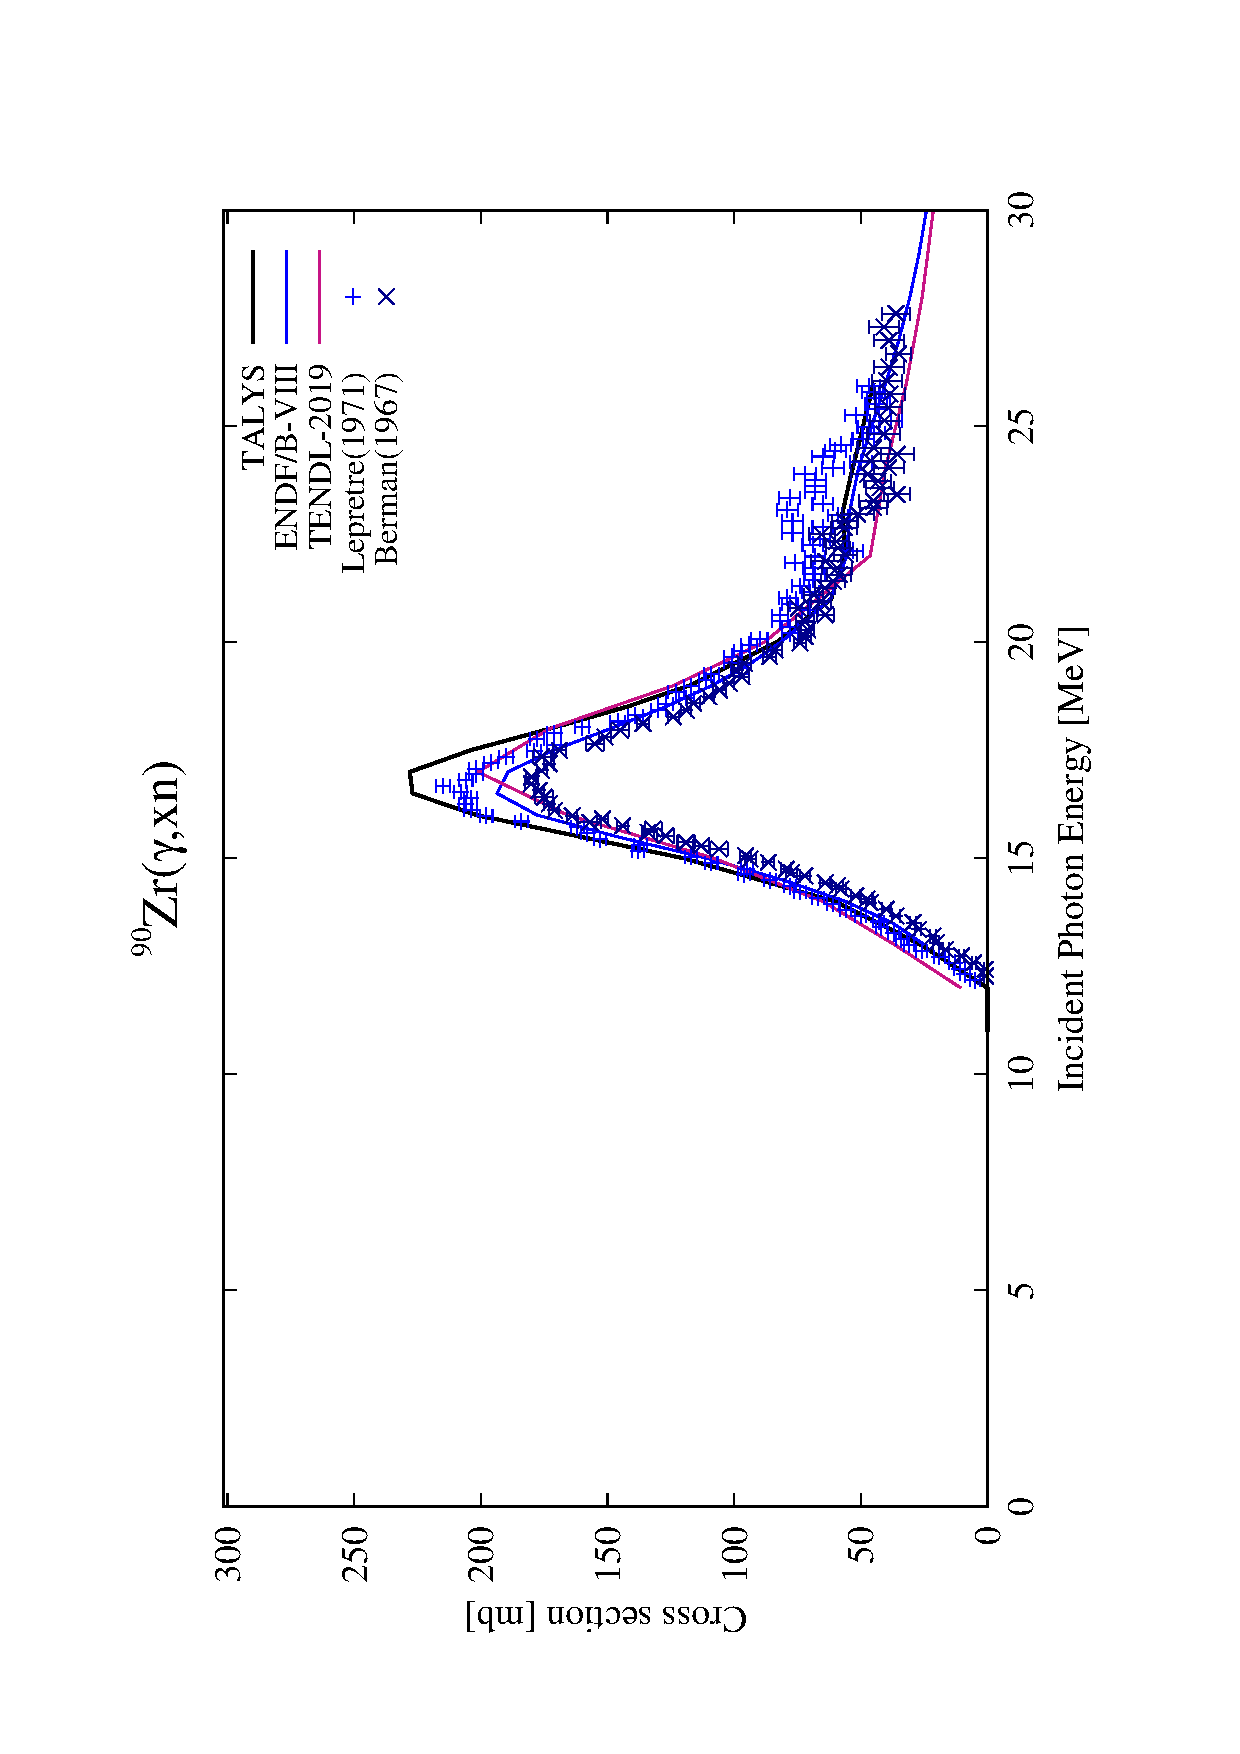
\includegraphics[scale=0.5,angle=270]{g-Zr090-xs}
\caption{Photonuclear reaction on ${}^{90}$Zr. Experimental data are obtained
from  Berman et al.~\protect\cite{Berman1967}.}
\label{zr090gn}
\end{figure}
